\section{Перечислимые множества.Теорема об эквивалентных определениях перечислимого множества.}
\begin{definition} Множество $A \subset \Sigma^*$ \textbf{перечислимо}, если $A=rng(f)$, где $f$ вычислима.
\end{definition}
Интуитивно это значит следующее: $f: \mathbb{N} \to \Sigma^*$ переводит какие-то натуральные числа в $f(n)$, при
этом мы получаем перечисление $x_{0}$, $x_{1}$, $x_{2}$... значений функции, которое и будет являться нашим
множеством $A$.

\begin{quote} {\textbf{Утверждение: }}
	Из разрешимости следует перечислимость.
	\par Действительно, если $A$ разрешимо, то можно вычислить характеристическую функцию $\chi_{A}(x)$, тогда положим
	$\chi^*_{A}(x)$ := $1$, если вычислили  $\chi_{A}(x)$ и получили $1$. В другом случае зациклимся. Построенная
	функция является вычислимой, определена на всех элементах множества $A$ и не определена иначе. Значит, $A$
	перечислимо.
\end{quote}
\begin{theorem}[эквивалентные определения перечислимого множества]
	\begin{enumerate}
		\item $A$ перечислимо;
		\item $A = \varnothing $ или $A = rng(f)$, где f -- тотально вычислимая функция;
		\item $A = \dom(f)$, где $f$ - вычислимая;
		\item Вычислима
			\begin{equation*}
				\chi^*_{A}(x) = 
				\begin{cases}
					\text{1, если $x \in A$}\\
					\text{не определена, иначе}
				\end{cases}
			\end{equation*}
		\item $A = \{\,x\mid\exists y <x,y> \in B,\}$, где $B$ - разрешимо. Это можно мыслить как проекцию на
			первую координату.
	\end{enumerate}
\end{theorem}
\begin{proof}
	\par2)$\Rightarrow$1), 4)$\Rightarrow$3) очевидно.
	\par3)$\Rightarrow$4) $A=\dom(f)$. Рассмотрим машину Тьюринга $M$, соответствующую $f$. Напишем новую машину
	Тьюринга $M'$, которая делает следующее: $M'$ работает как $M$, если же $M$ останавлвается, то мы стираем то,
	что было на ленте и пишем там $f$. $M'$ вычислит $\chi^*_{A}(x)$.  
	\par3)$\Rightarrow$5) Рассмотрим машину $M_{f}$, которая вычисляет $f: \dom(f)=A$ и рассмотрим множество $B =
	\{\,<x,y>\mid M_{f}(x)\mbox{ останавливается за }\leq y\mbox{ шагов }\,\}$. $B$ - разрешимо. Почему?
	Неформальный алгоритм звучит следующим образом: нам на входе дана пара $<x,y>$, запускаем машину $M_{f}$ и
	выполняем $y$ шагов. По паре можно понять, остановится ли работа машины $M_{f}$ и когда.
	\par $x \in A = \{\,x\mid <x,y> \in B \,\} \iff M_{f}$ останавливается $\iff \exists y <x,y> \in B $.
	\par5)$\Rightarrow$2) Пусть $A = \{\,x\mid \exists y <x,y> \in B\,\}$, $B$ - разрешимо. Допустим, что $A \neq
	\varnothing$. Выберем $a_{0} \in A$ и построим функцию $\varphi: \mathbb{N} \to \mathbb{N}$ такую, что 
	\begin{equation*}
		\varphi(n) = 
		\begin{cases}
			a_{0}\text{, если $n=<x,y> \notin B$}\\
			l(n)\text{, если $n=<x,y> \in B$ (l(n)=x, так как это проекция)}.
		\end{cases}
	\end{equation*}
	Она вычислима. $x \in A \iff \exists n (l(n)=x \land n \in B) \Rightarrow$ вычислима.
	\par1)$\Rightarrow$4) $A = rnd(f)$;дана машина $M_{f}$. Для данного $n$ = 0, 1, 2,... выполним $l(n)$ шагов
	вычисления функции $f(r(n))$ (теперь проекция на вторую координату), то есть $M_{f}(r(n))$, где $n = <l(n),
	r(n)>$. Если какое-то вычисление завершено и $f(r(n))=x$ (какому-то числу), то возьмём 1 на нём в качестве
	ответа. Схема обхода такова: \\ 
	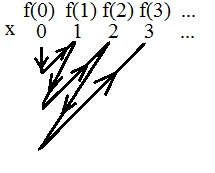
\includegraphics{S0RbSSTG2_4[1].jpg}
\end{proof}
